%%% The BEGINNING ~~~~
%%
% ~ Writes FPGP--MainText | By Filipe G. VIEIRA & George PACHECO



%% Preamble Settings %%

% Defines document class and paper size ~
\documentclass[twoside, british, a4paper]{article}

\usepackage{amsmath}
\usepackage{amsfonts}
\usepackage{amssymb,upref}
\usepackage{tgheros}
\usepackage{tgtermes}
\usepackage{anyfontsize}
\usepackage{enumitem}
\usepackage{subfig}
\usepackage{siunitx}
\usepackage{balance}
\usepackage{float}

% Fixes margins ~
\usepackage{geometry}
\geometry{reset,ignoreall,
  textheight = 253mm,
  textwidth = 175mm,
  bottom = 21mm,
  inner = 17.5mm,
  footskip = 8mm,
  headsep = 5mm,
  headheight = 10pt}
\usepackage[english]{babel}
\usepackage[utf8]{inputenc}
\usepackage{fancyhdr}
\renewcommand{\headrule}{}
\renewcommand{\footrule}{}

\setlength{\skip\footins}{1.75pc plus 5pt minus 2pt}
\def\footnoterule{
\kern-3mm \hrule height .5pt \kern -.4pt 
\kern 1mm}

\pagestyle{fancy}
\fancyhead[L]{Feral Pigeon Genomics}
\fancyhead[R]{Pacheco et al. 2021}
\fancypagestyle{firstpage}{%
\fancyhf{}
\lhead{}
\rhead{}}

% Loads packages for images ~
\usepackage{graphicx}
\usepackage{rotating}

% Loads packages for comments ~
\usepackage{verbatim}
\usepackage[hang, flushmargin]{footmisc}

% Loads packages for tables ~
\usepackage{float}
\usepackage{multirow}
\usepackage{lmodern}
\usepackage{textcomp}
\usepackage[utf8]{inputenc}
\usepackage[TU]{fontenc}

% Listing of source code ~
\usepackage{listings}
\usepackage{color}
\definecolor{dkgreen}{rgb}{0,0.6,0}
\definecolor{gray}{rgb}{0.5,0.5,0.5}
\definecolor{mauve}{rgb}{0.58,0,0.82}
\lstset{
  frame = tb,
  language = sh,
  aboveskip = 3mm,
  belowskip = 3mm,
  showstringspaces = false,
  columns = flexible,
  basicstyle = {\small\ttfamily},
  numbers = none,
  numberstyle = \tiny\color{gray},
  keywordstyle = \color{blue},
  commentstyle = \color{dkgreen},
  stringstyle = \color{mauve},
  breaklines = true,
  breakatwhitespace = true,
  tabsize = 3}
  
% Changes caption starting text ~
\renewcommand{\figurename}{Supplementary Figure}
\renewcommand{\tablename}{Supplementary Table}

% Loads packages for typing ~
\usepackage{lettrine}
\pdfmapfile{=montserrat.map} 
\renewcommand{\LettrineFont}{
  \fontfamily{iwonal}\fontsize{30}{30}\selectfont
  \color[rgb]{0.25,0.25,0.25}}
\usepackage{marvosym}

\newcommand\myhline{%
  \noindent\rule[.5pt]{\linewidth}{.4pt}\par%
}

\newcommand{\myheaders}[1] {\noindent{\normalsize{\fontfamily{bch}\selectfont{\textbf{#1}}}}}
\newcommand{\mysubheaders}[1] {\noindent{\fontfamily{bch}\selectfont{\textbf{#1}}}}
\newcommand{\mytext}[1] {\noindent{\fontfamily{bch}\selectfont{#1}}}

% Figure captions
\usepackage{caption}
\DeclareCaptionFont{cfs}{\fontsize{8.5}{10.25}\selectfont}
\DeclareCaptionLabelSeparator{vline}{\;|\;}
\captionsetup{
 labelsep=vline, 
 font={sf,cfs}, 
 labelfont={cfs,bf},
 belowskip=-12pt}
\newcommand{\figurecaption}[2]{\caption[#1]{\textbf{#1.} #2}}
\usepackage{hyperref}
\usepackage[dvipsnames]{xcolor}
\definecolor{mycolor}{HTML}{F7F8E0}
\definecolor{myorange}{RGB}{245,156,74}
\hypersetup{
  colorlinks=true,
  urlcolor=-myorange}

\usepackage{fontawesome}

\usepackage[nopar]{lipsum}
\newcommand\blfootnote[1]{%
  \begingroup
  \renewcommand\thefootnote{}\footnote{#1}%
  \addtocounter{footnote}{-1}%
  \endgroup}

% Loads packages for bibliography ~
\usepackage[
backend = biber,
style = nature,
sorting = ynt
]{biblatex}
\addbibresource{FPG--MainText.bib}

\usepackage{blindtext}
\usepackage{multicol}

%% Starts Document %%

% Starts document ~
\begin{document}\thispagestyle{empty}

%\twocolumn[
%\begin{@twocolumnfalse}

% Sets title ~
\LARGE{\bfseries{\fontfamily{cmr}\color[rgb]{0.25,0.25,0.25}\noindent{On the Origin and Spread of Feral Pigeons}}} \\

% Sets authorship ~
\fontfamily{cmr} \small \noindent 
George Pacheco\,$^{1}$\textsuperscript{\faEnvelopeO},
Filipe G. Vieira\,$^{1}$,
Michael D. Martin\,$^{1}$,
Morten Tange Olsen\,$^{1}$,
Pavel Hulva\,$^{1}$,
Tânia de Freitas Raso\,$^{1}$,
Peter Njoroge\,$^{1}$,
Concepción Salaberria\,$^{1}$,
Isabel López-Rull\,$^{1}$,
Carles Lalueza-Fox\,$^{1}$,
Oscar Ramírez\,$^{1}$,
María C. Ávila-Arcos\,$^{1}$,
Patricia Rosas Escobar\,$^{1}$,
Rui Faria\,$^{1}$,
Miguel Carneiro\,$^{1}$,
Graciela Sotelo\,$^{1}$,
Jóhannis Danielsen\,$^{1}$,
Nizar Haddad\,$^{1}$,
Fares Khoury\,$^{1}$,
Roi Dor\,$^{1}$,
Ali Halajian\,$^{1}$,
María Belén Arias\,$^{1}$,
Oliver Krone\,$^{1}$,
Susanne Auls\,$^{1}$,
Sampath S. Seneviratne\,$^{1}$,
Kajanka Mathiaparanam\,$^{1}$,
Michael Bunce\,$^{1}$,
Megan L. Coghlan\,$^{1}$,
Jon Fjeldså\,$^{1}$ \&
M. Thomas P. Gilbert\,$^{1}$\textsuperscript{\faEnvelopeO} \\
\myhline

% Sets affiliations ~
\blfootnote{\scriptsize{\fontfamily{cmr}$^1$Section for Evolutionary Genomics, The GLOBE Institute, Faculty of Health and Medical Sciences, University of Copenhagen, Copenhagen, Denmark. $^1$Natural History Museum of Denmark, University of Copenhagen, Øster Voldgade 5–7, 1350 Copenhagen, Denmark. $^1$NTNU University Museum, Norwegian University of Science and Technology, Trondheim, Norway $^1$Department of Zoology, Charles University, Prague, Czech Republic. $^1$Departamento de Patologia, Faculdade de Medicina Veterinária e Zootecnia, Universidade de São Paulo, São Paulo, Brazil. $^1$Ornithology Section, Department of Zoology, National Museums of Kenya, Nairobi, Kenya. $^1$Centro de Investigación en Ecosistemas, Universidad Nacional Autonoma de Mexico, Michoacan, Mexico. $^1$Departamento de Ecología Evolutiva, Museo Nacional de Ciencias Naturales, Madrid, Spain. $^1$Avian Evolution Node, Department of Zoology and Environment Sciences, University of Colombo, Colombo, Sri Lanka. $^1$Institute of Evolutionary Biology, Universitat Pompeu Fabra, Barcelona, Spain. $^1$Department of Animal and Plant Sciences, University of Sheffield, Sheffield, UK. $^1$Centro de Investigação em Biodiversidade e Recursos Genéticos, Universidade do Porto, Vairão, Portugal. $^1$Institute of Evolutionary Biology, Department of Experimental and Health Sciences, University, Pompeu Fabra, Spain. $^1$Departamento de Biologia, Faculdade de Ciências, Universidade do Porto, Porto, Portugal. $^1$University of the Faroe Islands, Tórshavn, Faroe Islands. $^1$National Center for Agricultural Research and Extension, Al-Baqah, Jordan. $^1$Department of Biology and Biotechnology, American University of Madaba, Madaba, Jordan. $^1$Department of Zoology, Tel Aviv University, Tel Aviv, Israel. $^1$Natural History Museum, Imperial College of London, London, United Kingdom. $^1$Department of Biodiversity, Turfloop Campus, University of Limpopo, Polokwane, South Africa. $^1$Department of Wildlife Diseases, Leibniz Institute for Zoo and Wildlife Research, Berlin, Germany. $^1$Vetgenomics SL, Edifici Eureka, Campus UAB, Barcelona, Spain. $^1$Trace and Environmental DNA (TrEnD) Laboratory, Department of Environment and Agriculture, Curtin University, Perth, Australia.\\ \textsuperscript{\faEnvelopeO}Correspondence should be addressed to \href{mailto:ganpa@aqua.dtu.dk}{ganpa@aqua.dtu.dk} (G.P.) \& \href{mailto:tgilbert@sund.ku.dk}{tgilbert@sund.ku.dk} (M.T.P.G.)}}

% Sets abstract text ~
\mytext{\noindent{\textbf{The rock pigeon (\textit{Columba livia} Gmelin, 1789) is presumed native to the Mediterranean, Saharo-Arabian and Eastern Oriental regions, and is believed to have been domesticated in the Middle East in the early Neolithic. At some point during the domestication process, the first feral pigeons arose, whose populations subsequently undertook a remarkable expansion that has resulted in them being found today across almost the entire global urban landscapes. Indeed the spread of these feral birds has been so prolific, that it raises questions about whether any true wild rock pigeon colonies still exist, or whether they have been admixed with, or even fully replaced, by feral birds? While several studies have investigated the complex evolutionary history of pigeon breeds, none have yet addressed the question of pigeon feralisation, and how this evolutionary process might be jeopardizing the species’ status as a wild entity. In this study, we generated and analysed a genomic dataset produced using the Genotyping-by-Sequencing (GBS) method of 450 feral pigeons sampled across 41 worldwide localities. Our analyses reveal that the global feral pigeon population can be divided into four major groups, each exhibiting different levels of genetic diversity and contamination with domesticated genotypes. We also find signs of strong population structure, including very divergent clades of what seems to be relatively wild populations. Lastly, we find evidence of human-mediated dispersal through past colonial links.}}} \\

\hfill\break

% Introduction %

\begin{multicols}{2}
\lettrine[findent=2pt]{\textbf{A}}{ }\mytext{rchaeological evidence suggests that the rock pigeon (\textit{Columba livia} Gmelin, 1789), and in particular the (\textit{C. l. livia}) subspecies, was first domesticated during the Neolithic period in the Middle East, probably via a commensal pathway2. While it was initially exploited as a source of food and fertiliser, later on, the extent of its service to humankind spanned a wider variety of roles, including incorporation into religious rituals, a tool for communication, a source of medicine, and even as a navigation aid3. Furthermore, in addition to its practical functional roles, and in parallel with many other domestic animals such as dogs, chickens and cats, the eighteenth century witnessed an explosion of interest in the development of so-called fancy breeds. Such interest led to the establishment of numerous pigeon breeds, of which over 230 are currently recognised by the \textit{American National Pigeon Association} (NPA; \mytext{\url{www.npausa.com}}). Artificial selection in modern breeds resulted in a truly fabulous amount of phenotypic diversity, which has long attracted the attention of scholars, and even formed a cornerstone of Darwin’s nascent thoughts on his famous theory concerning the evolutionary processes \cite{pacheco_darwins_2020}.} \\
\indent\mytext{The history of the pigeon domestication has also been tightly coupled with a correlative evolutionary process—feralisation. The process of feralisation is thought to have begun through domestic pigeons escaping from captive stocks (kept within Europe, North Africa and Western Asia). As to the ecological niche of their wild ancestors, feral pigeons tend to utilise hardscape habitats as urban analogues of rocks/cliffs (Lundholm and Richardson, 2010) and become a synurbic species (Francis and Chadwick, 2012). As with other feralised domesticates, the species experienced an extreme ecological range expansion much later in time, when during the modern colonial period they were transmitted to, and subsequent release across, almost all continents of the world, successfully populating extensive urban areas. Therefore, at present, the feral pigeon is ubiquitous across the world’s urban landscapes, where it is often considered a pest species requiring active management. Furthermore, given that both domestic and feral pigeons can almost certainly still interbreed with their wild ancestor, it has been proposed that in regions of co-occurrence, the wild rock pigeon gene pools (and thus their integrity as a natural species) might be to some extent contaminated with domestic genotypes as has been demonstrated for other domestic species5,6.} \\
\indent\mytext{Although studies aiming to shed light on the genomic relationships among pigeon breeds have been conducted7–9, fundamental questions concerning today's feral pigeon populations have yet to be addressed in depth. These include i) which breeds principally contributed to the formation of the feral pigeon populations, and ii) which are the genomic relationships among these populations. Additionally, in light of the global expansion of both domestic stocks and feral populations during the past few centuries, and a third key question is iii) whether the wild rock pigeon has undergone a process of genomic extinction as seen with the wild ancestors of other domesticates6,10.} \\
\indent\mytext{In this study, we employed the Genotyping-by-Sequencing (GBS) method to generate a genomic dataset for 450 free-living pigeons from 41 localities covering a worldwide distribution, as well as XXX pigeons representing other subspecies/species??. We use this dataset to reconstruct the phylogenetic relationships among these populations, as well as to investigate their patterns of both genetic structure and diversity revealed by analyses of MDS, Admixture and population genetics statistics.} \\
\indent\mytext{We hypothesize that populations inhabiting remote localities within the believed natural range will show the lowest levels of contamination with domestic genotypes, while those populations inhabiting urban localities within the believed natural range will have moderate signals of admixture with domesticates. Besides, those populations outside the natural range will show the highest levels of influence by domestic genotypes, and, given that these populations were formed through human-mediated dispersals, we also expect that there will be a signal linking former colonies-colonizers relationships (e.g. London and Johannesburg).} \\

% Results %

\myheaders{Results} \\
\mysubheaders{Sampling effort.} \mytext{To investigate the genomic patterns of current pigeon populations of different evolutionary histories, we intentionally targeted our sampling to cover four distinct categories (Figure 1). Furthermore, to help root the evolutionary relationships between these groups, we also included a small number of individuals representing the Columba livia intermedia (Strickland, 1844) subspecies. Specifically in this regard, we sampled five populations from Sri Lanka, where two of them were from urban localities (Colombo and Trincomalee), one was from a Conservation National Park (Pigeon Island) and two others were captive populations maintained by local breeders (Wattala and Wellawatte) (Supplementary Fig. 1). To check for data reproducibility, we sequenced two of the samples twice (Tehran\textunderscore16-GBS and Perth\textunderscore02-GBS) to serve as replicates. Finally, to serve as external outgroups, we also generated data from five samples of (\textit{Columba palumbus Linnaeus}, 1758) captured in Copenhagen (Denmark), one captive sample of (\textit{Streptopelia risoria} Linnaeus, 1758), and additionally incorporated previously published whole genome resequence data from a Columba rupestris8. (we also included the WGS library to serve as another replicate) (Supplementary Spreadsheet).}

\mysubheaders{Sequencing data and filtering.} \mytext{We generated 1,062,089,639 reads using the (GBS) method11 from all 488 samples. The percentage of GBS chimeric reads removed ranged from 0.034\% to 4.65\% (mean of 0.69\%) per sample. Based on the presence/absence heatmap, we excluded 10 samples alongside the 6 blanks from downstream analyses (Supplementary Fig. 2). The sequencing depths across the regions of interest ranged from 0.069X to 19.97X (mean of 2.32X) (Supplementary Spreadsheet), with 68.86\% of the predicted cut-sites yielding no data for any sample. This pattern is not unexpected with GBS data and derives from differences in sequencing effectiveness at different sites in the genome, and has also been observed in other GBS data from pigeons9. Moreover, based on the Global Depth (GD) results (Supplementary Fig. 3), we elected to run subsequent downstream analyses on only sites that have GD of at least 150X.} \\

\mysubheaders{Population genetics statistics.} \mytext{Hybridisation between domestic lineages and their respective wild ancestors is an issue of conservation importance as the genomic integrity of wild lineages can be disturbed by contamination with domestic genotypes, either through direct admixture with purebred lineages or through indirect contact with feral stocks5,12. To shed light on the levels of potential domestic contamination, as well as isolation among the sampled populations, we calculated several population genetics estimates for the different pigeon populations as well as Fst levels between them. First, we calculated the observed levels of heterozygosity (Ho) for each sample present in Dataset 1 (all samples). Among the free-living pigeon individuals, the Ho ranged from 0.1157\% to 0.2747\% (average of 0.2231\%) (Supplementary Spreadsheet), with considerable variation within each population and the occurrence of several outliers (Supplementary Fig. 5). On the other hand, the Ho ranged from 0.1818\% to 0.2389\% (average of 0.2176\%) among the five C. palumbus samples.} \\
\indent \mytext{Moreover, we calculated the nucleotide diversity ($\pi$), Watterson's $\Theta$ ($\Theta$w), and Tajima’s D across the pigeon genome for the 35 populations that had five or more individuals (the Crete population was also included due to its relevance), as these genetic estimates only apply for population data (for the 2 replicate samples only the ones with higher coverage were used) (Supplementary Fig. 6). $\Pi$ ranged from 0.001764 to 0.003080 (average: 0.002584; C. palumbus: 0.002427); $\Theta$w ranged from 0.001507 to 0.003168 (average: 0.002483; C. palumbus: 0.002644) and the Tajima’s D  ranged from -0.643739 to 0.854540 (average: 0.248505; C. palumbus: -0.413195). Interestingly, the values calculated for the five C. palumbus individuals in our study were lower than expected for a wild species, but we believe that the fact we analysed synanthropic individuals might have prevented us from accessing the true values for this species (Supplementary Spreadsheet.} \\
\indent \mytext{We next elected to calculate the pairwise Fst between populations to provide preliminary insights into the relationships between the different populations. A heatmap plotted using this data, after excluding the populations of Tel Aviv Colony and C. palumbus that showed extremely high levels of divergence (Supplementary Fig. 7), clearly shows that three clusters are recovered. The first contains populations from relatively isolated regions within the natural range  (Pigeon Island, Trincomalee, Torshavn, Crete, Sardinia, Vernelle, Wadi Hidan, Abadeh and Tehran). The second contains populations from mostly Europe and former colonies (Tel Aviv, Barcelona, Guimaraes, Lisbon, Berlin, Prague, Denver, London, Perth, Salvador, Copenhagen, Johannesburg and Salt Lake City). The third contains populations from Mexico (Santiago, San Cristobal de las Casas, Monterey, Tlaxcala de Xicohtencatl and Mexico City).} \\
\indent \mytext{Overall, we see a wide range of genetic diversity levels among the sampled populations, similar to both domesticated (e.g. duck breeds: 0.0020 to 0.0028) and wild species (e.g. mallard: 0.0040)13. Tajima’s D values show a general pattern of positive values, indicating population contractions, except for the populations from Tehran, Abadeh, Wadi Hidan, and Sardinia. Taken together, these results seem to group the current pigeon diversity into four groups, depending on the levels of genetic diversity (high, intermediate, or low), while the group with high levels of genetic diversity can be further subdivided depending on Tajima’s D values (positive or negative). These groupings are further supported by the Fst distances, which clearly form groups around the populations with both intermediate and high genetic diversity.} \\

\mytext{Even though the levels of genetic diversity can give initial valuable insights regarding the past history of a given population, it is also important to infer the evolutionary relationships among the current pigeon populations. For that, we conducted the first phylogenetic reconstruction for non-domestic pigeon populations. Specifically, we first performed a Neighbour-joining (NJ) phylogenetic analyses based on Dataset 1 to confirm the appropriateness of the outgroups available (Supplementary Fig. 8). Having confirmed that Columba rupestris is the most appropriate outgroup, we proceeded with a Maximum-likelihood (ML) phylogenetic analysis based on Dataset 2 (excluding S. risoria and C. palumbus). Overall, the ML phylogeny reconstructed reveals a strong phylogenetic structure across the different pigeon populations studied (Fig. 1). Despite the low bootstrap values (BS) recovered for the internal nodes (probably because the evolution of pigeons is not a truly bifurcating process), we delineated six main groups on our phylogeny based on geographical distribution and biological assumptions; Group A: The Pigeon Island and Trincomalee C. l. intermedia populations; Group B: Abadeh, Tehran, Crete, Sardinia, Vernelle and the Faroe Islands; Group C: Tel Aviv, Tel Aviv Colony and Wadi Hidan populations; Group D: Nairobi, Colombo, Lahijan, Nowshahr, Wellawatte and Isfahan populations; Group E: Guimaraes, Barcelona, Lisbon, Salvador, Tatui, Denver, Santiago, Tlaxcala de Xicohtencatl, Mexico City, Monterrey and San Cristobal de Las Casas populations; Group F: Jihlava, Prague, Berlin, Salt Lake City, Johannesburg, London, Cambridge, Perth and Copenhagen. Interestingly, the four individuals belonging to the Wattala population do not form a monophyletic group and are found scattered across the phylogeny.} \\
\mytext{It is noteworthy that Group A, as well as both the Faroe Islands and the Tel Aviv Colony populations, have 100\% of BS, with the former also having a very elongated branch length. Moreover, all the three replicates (namely, Crupestris_01, Tehran_16 and Perth_02) behave as expected, all clustering with 100\% of BS. Furthermore, although both the eight Wattala and Wellawatte captive populations were located within the Colombo region, these populations do not form a distinct clade together with the Colombo population with some Wattala individuals sitting on a rather different region of the phylogeny. As for the three captive populations included in our study, all 6 individuals belonging to the Tel Aviv Colony population form a clade with 100\% of BS and phylogenetic affinity with the Tel Aviv and the Hadi Hidan populations. The branch of this cluster is the longest across the entire phylogeny, in agreement with the fact that this colony has been maintained inbread for several generations.} \\

\end{multicols}

\begin{figure}[H]
\centering
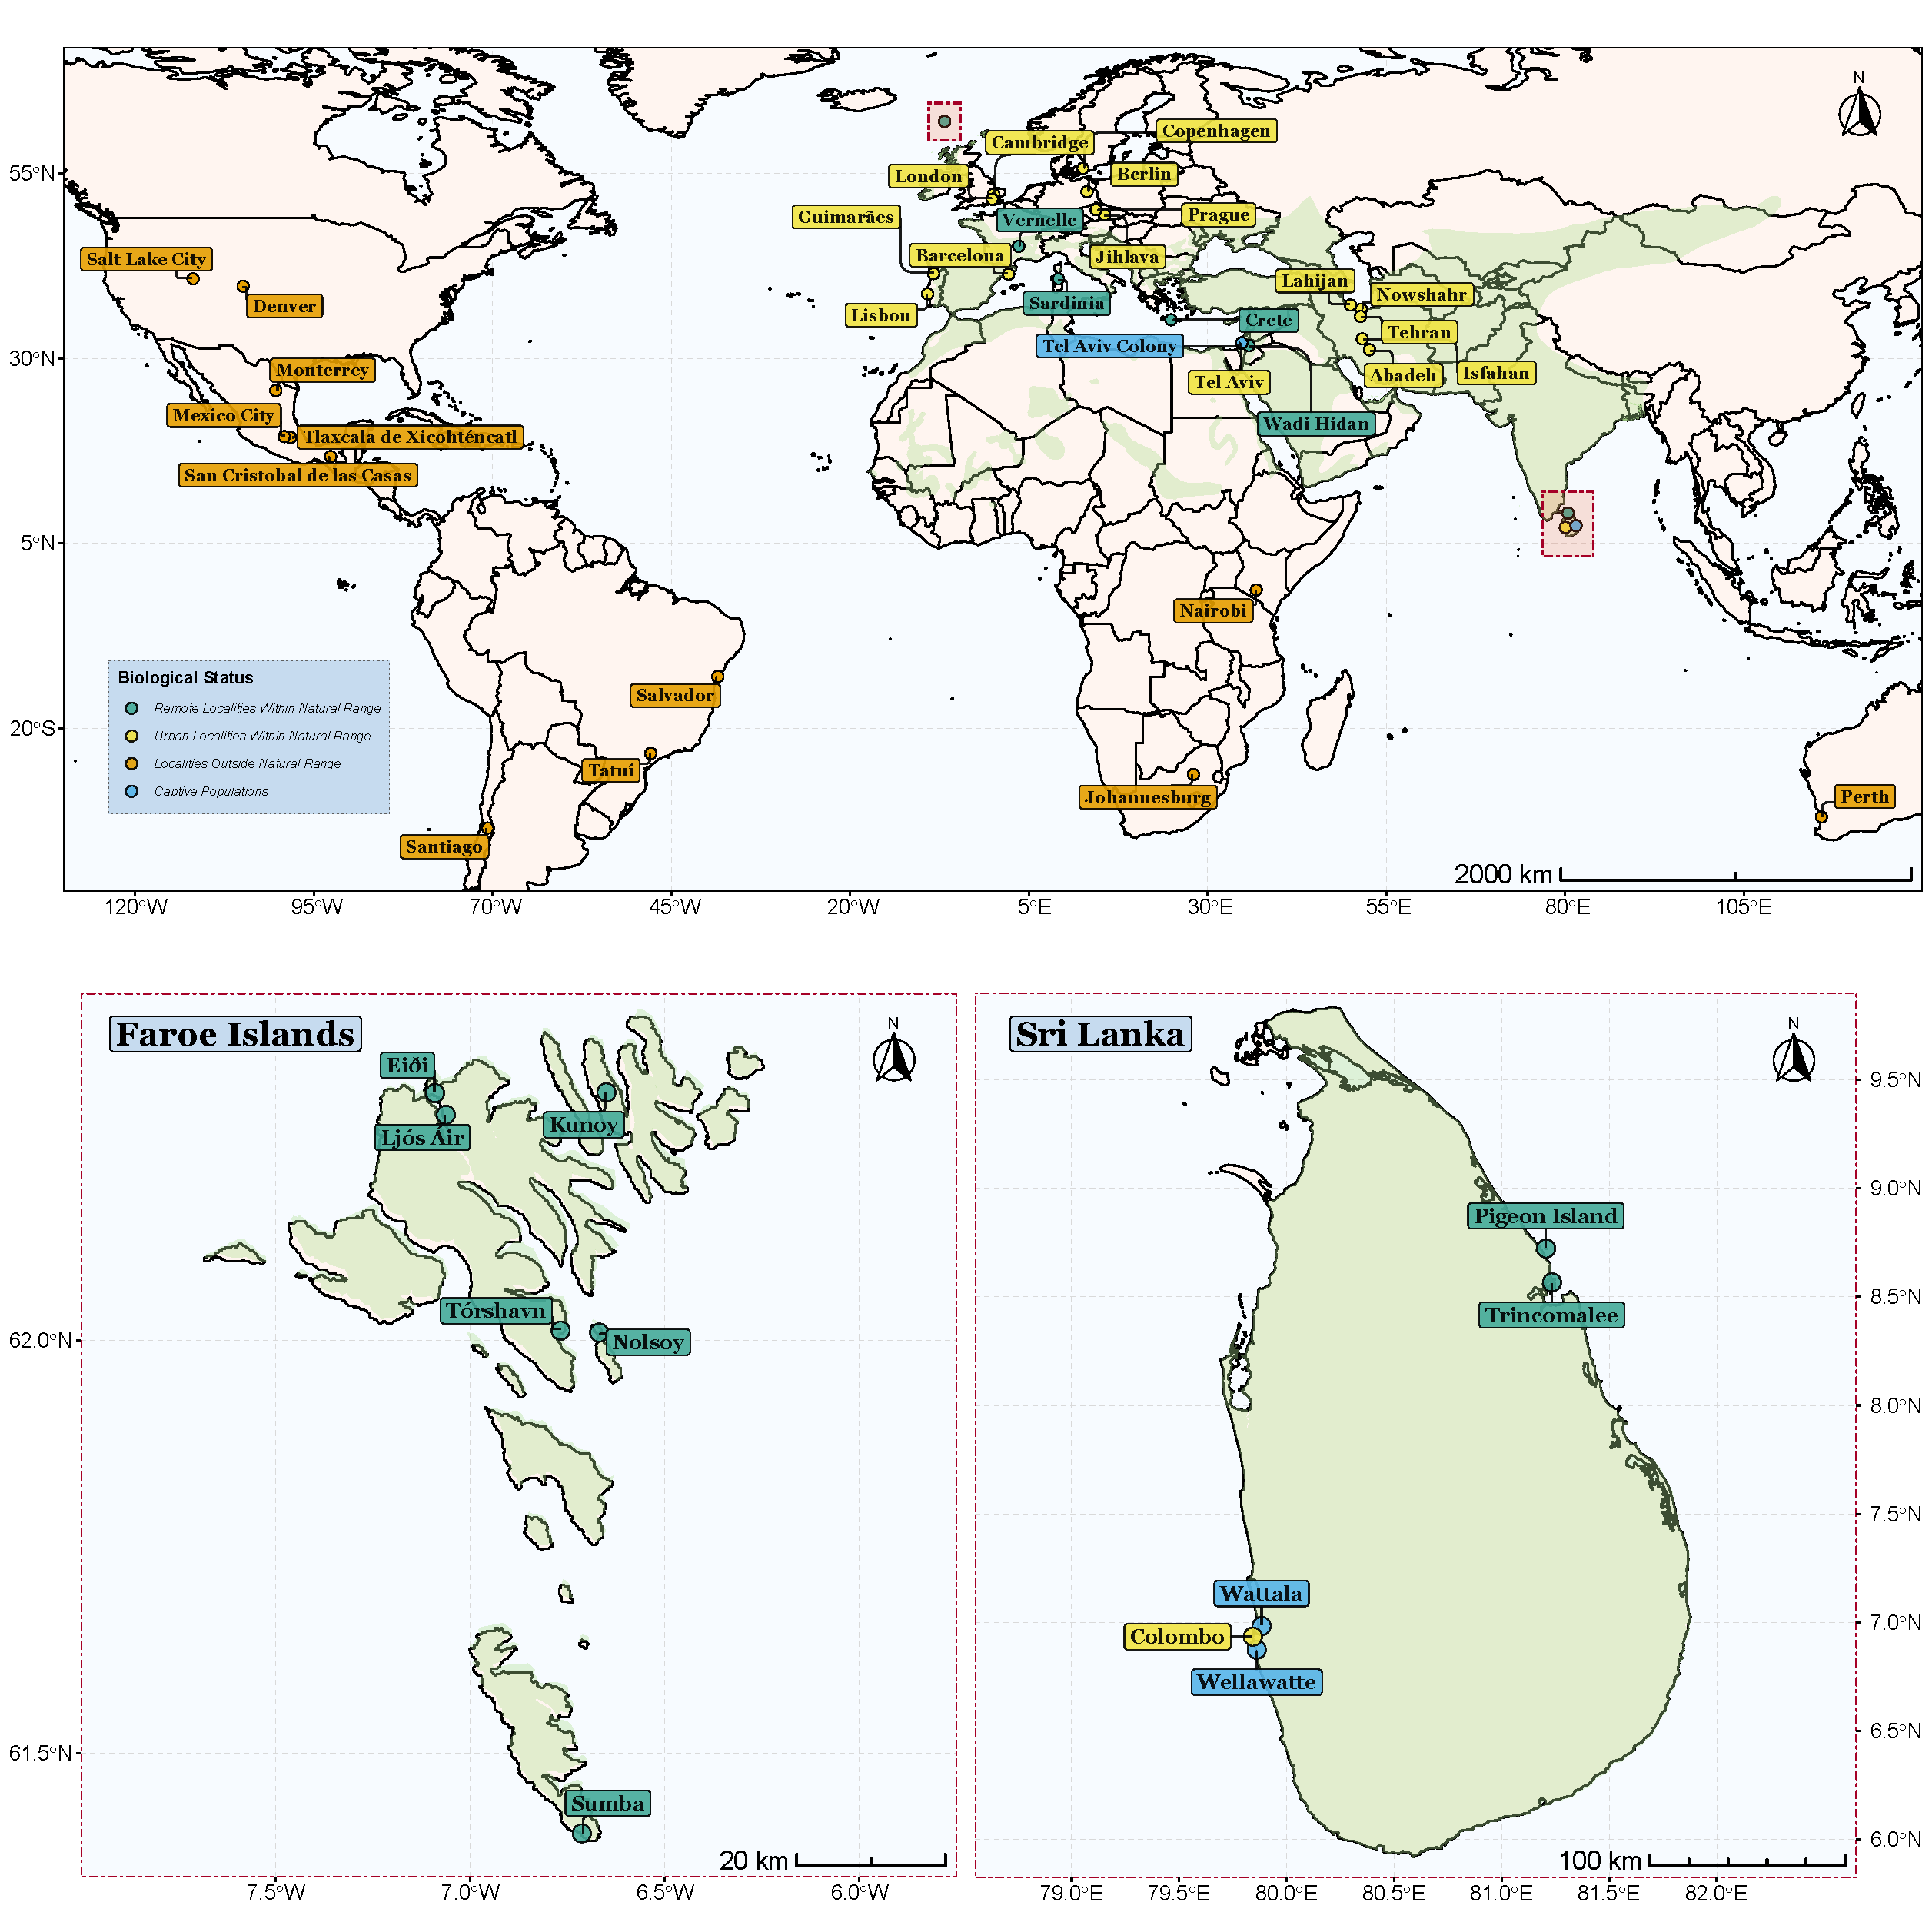
\includegraphics[width=1\textwidth]{../FPG--Plots/FPG--Map/FPG--Map.pdf}
\caption*{ \scriptsize \textbf{Fig. 1 Map of sampling effort.} This is a trial attempt.}
\label{MainText:FPGP--Map}
\end{figure}

\begin{multicols}{2}

\mysubheaders{Phylogenetic relationships among feral pigeon populations.}\\
\mysubheaders{Population structure among pigeon populations.}\\
\mysubheaders{Contribution of pigeon breeds to current non-domesticated populations.}\\

% Discussion %

\myheaders{Discussion} \\

% Methods %

\myheaders{Methods} \\

\mysubheaders{Sequencing data generation and processing.} \\
\mysubheaders{Data analysis.} \\
\mysubheaders{Population genetics statistics.} \\
\mysubheaders{Phylogenetic reconstruction.} \\
\mysubheaders{Inference of Population Structure.} \\
\mysubheaders{Contribution of pigeon breeds to current non-domesticated populations.} \\
\end{multicols}

\begin{figure}[!ht]
\centering
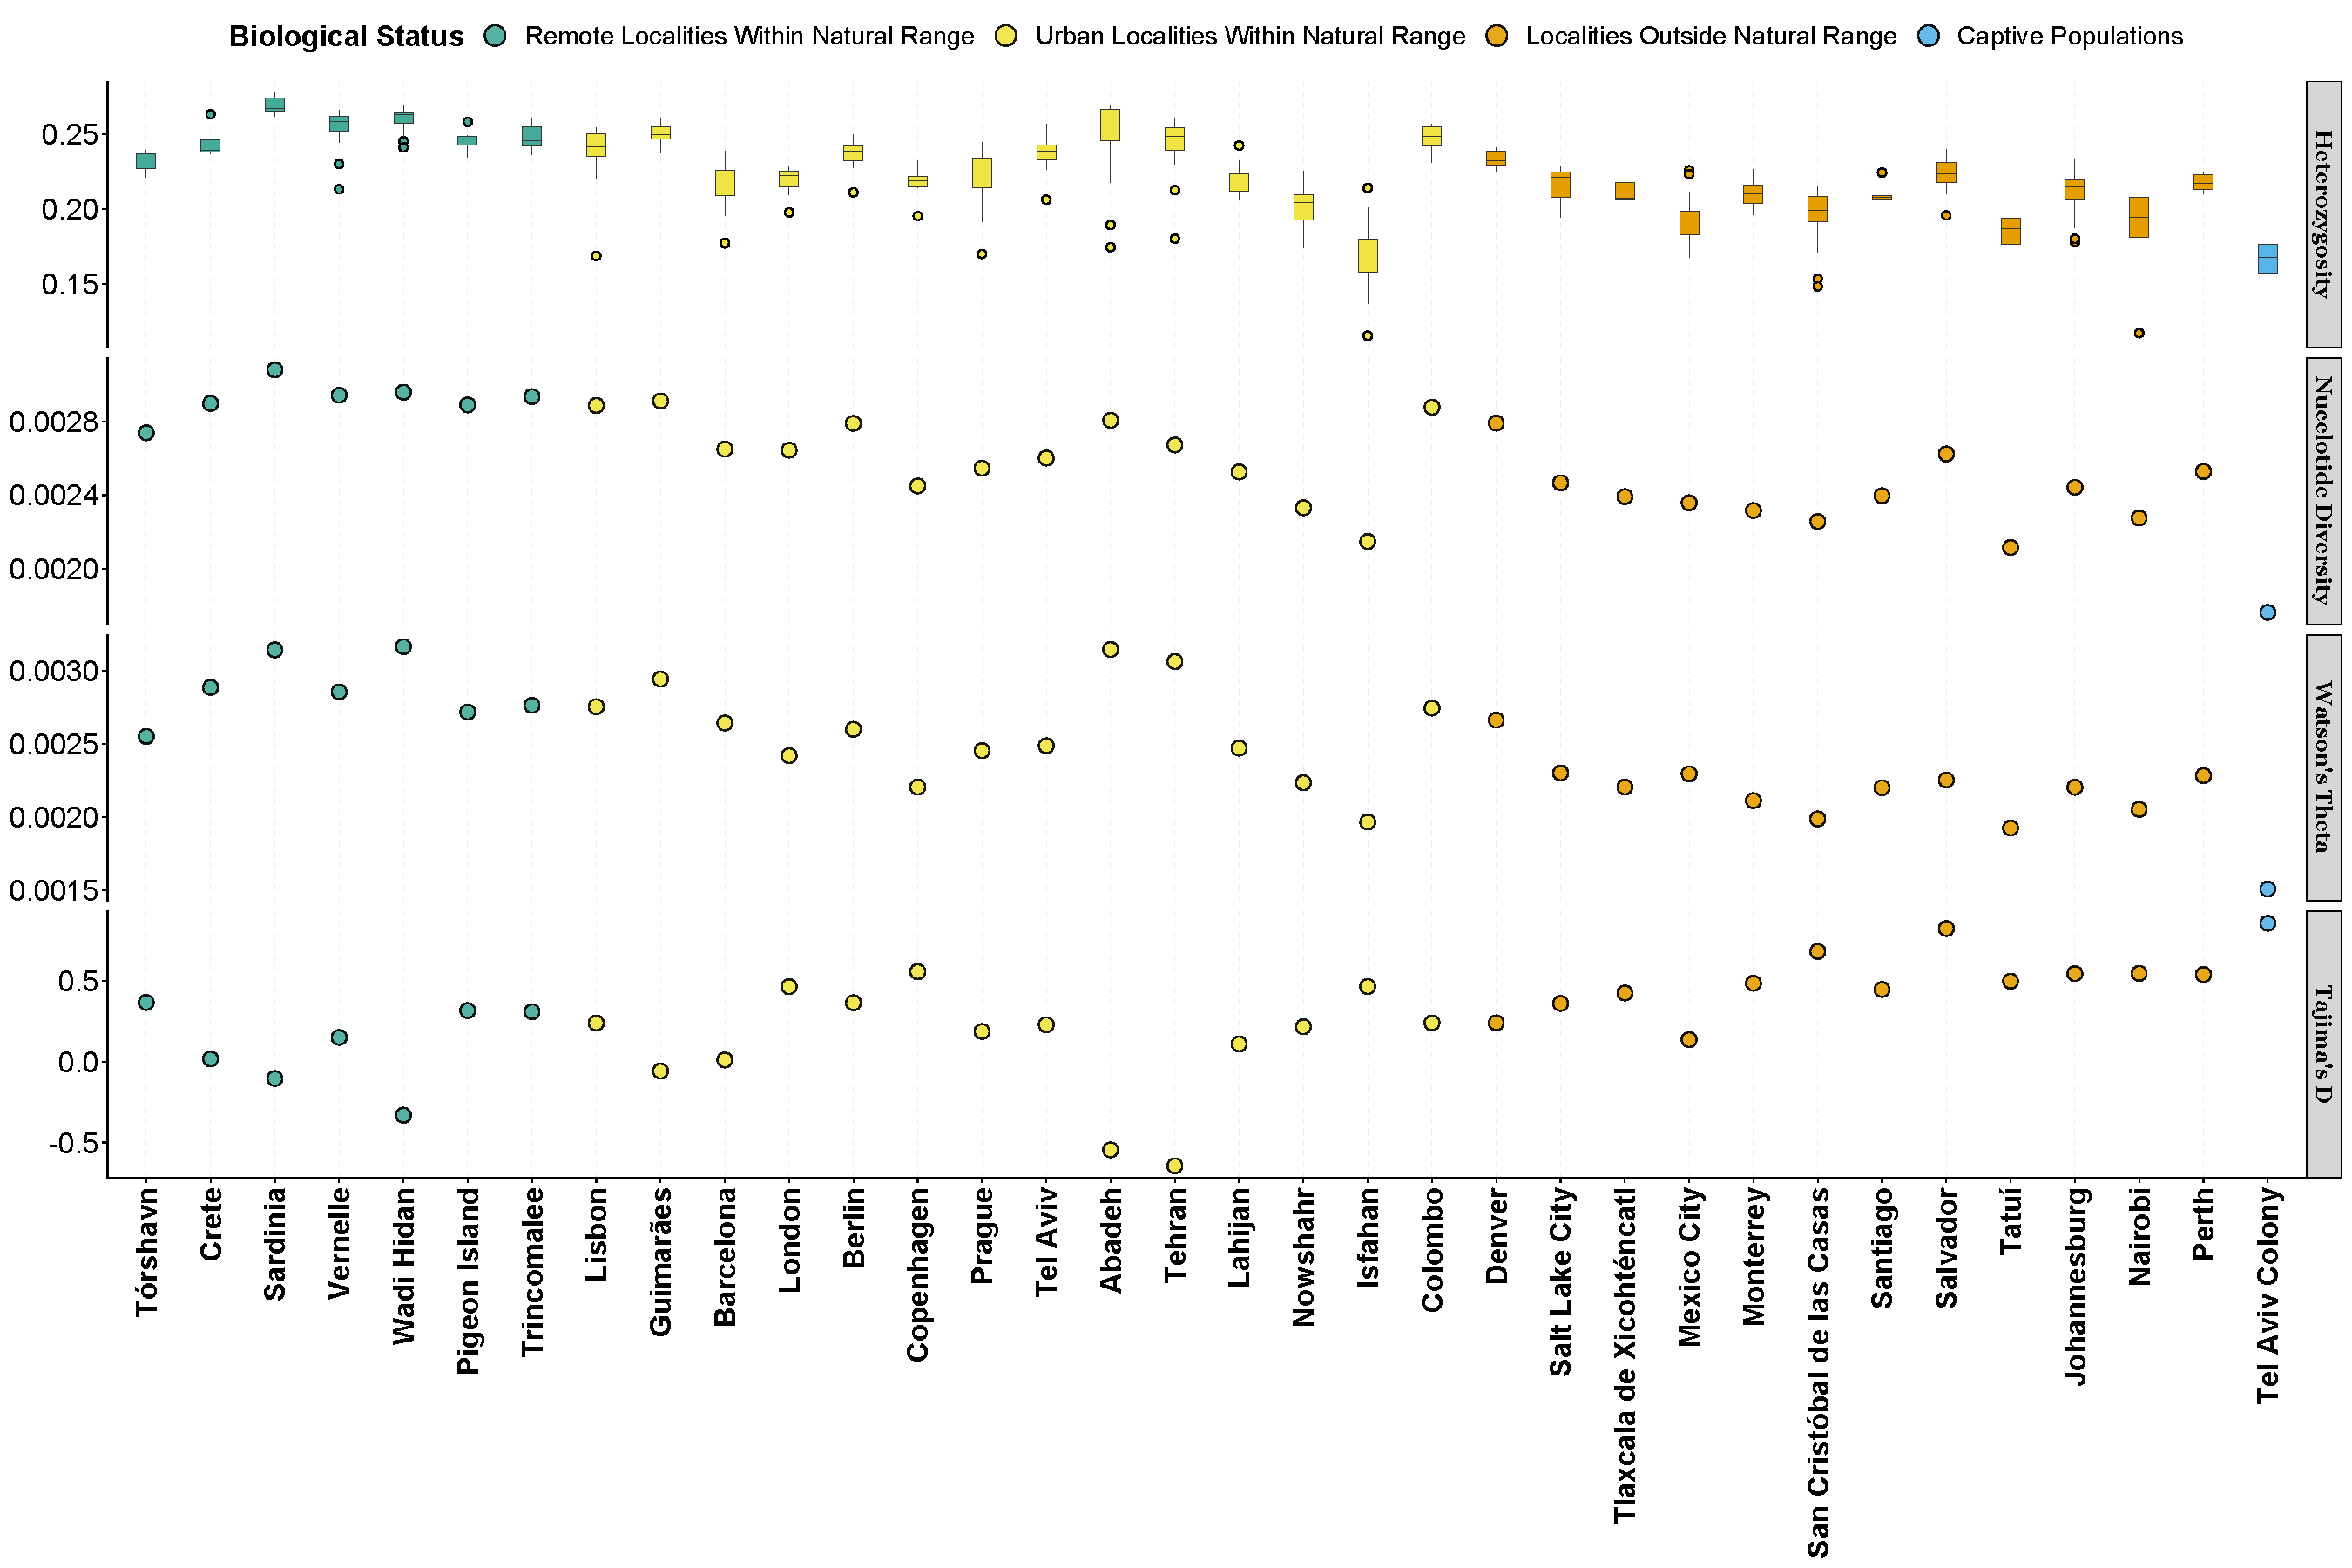
\includegraphics[width=1\textwidth]{../FPG--Plots/FPG--PopGenEstimates/FPG--PopGenEstimates.pdf}
\caption*{ \scriptsize \textbf{Fig. 2 Map of sampling effort.} This is a trial attempt.}
\label{MainText:FPGP--PopGenEstimates}
\end{figure}

\begin{figure}[!ht]
\centering
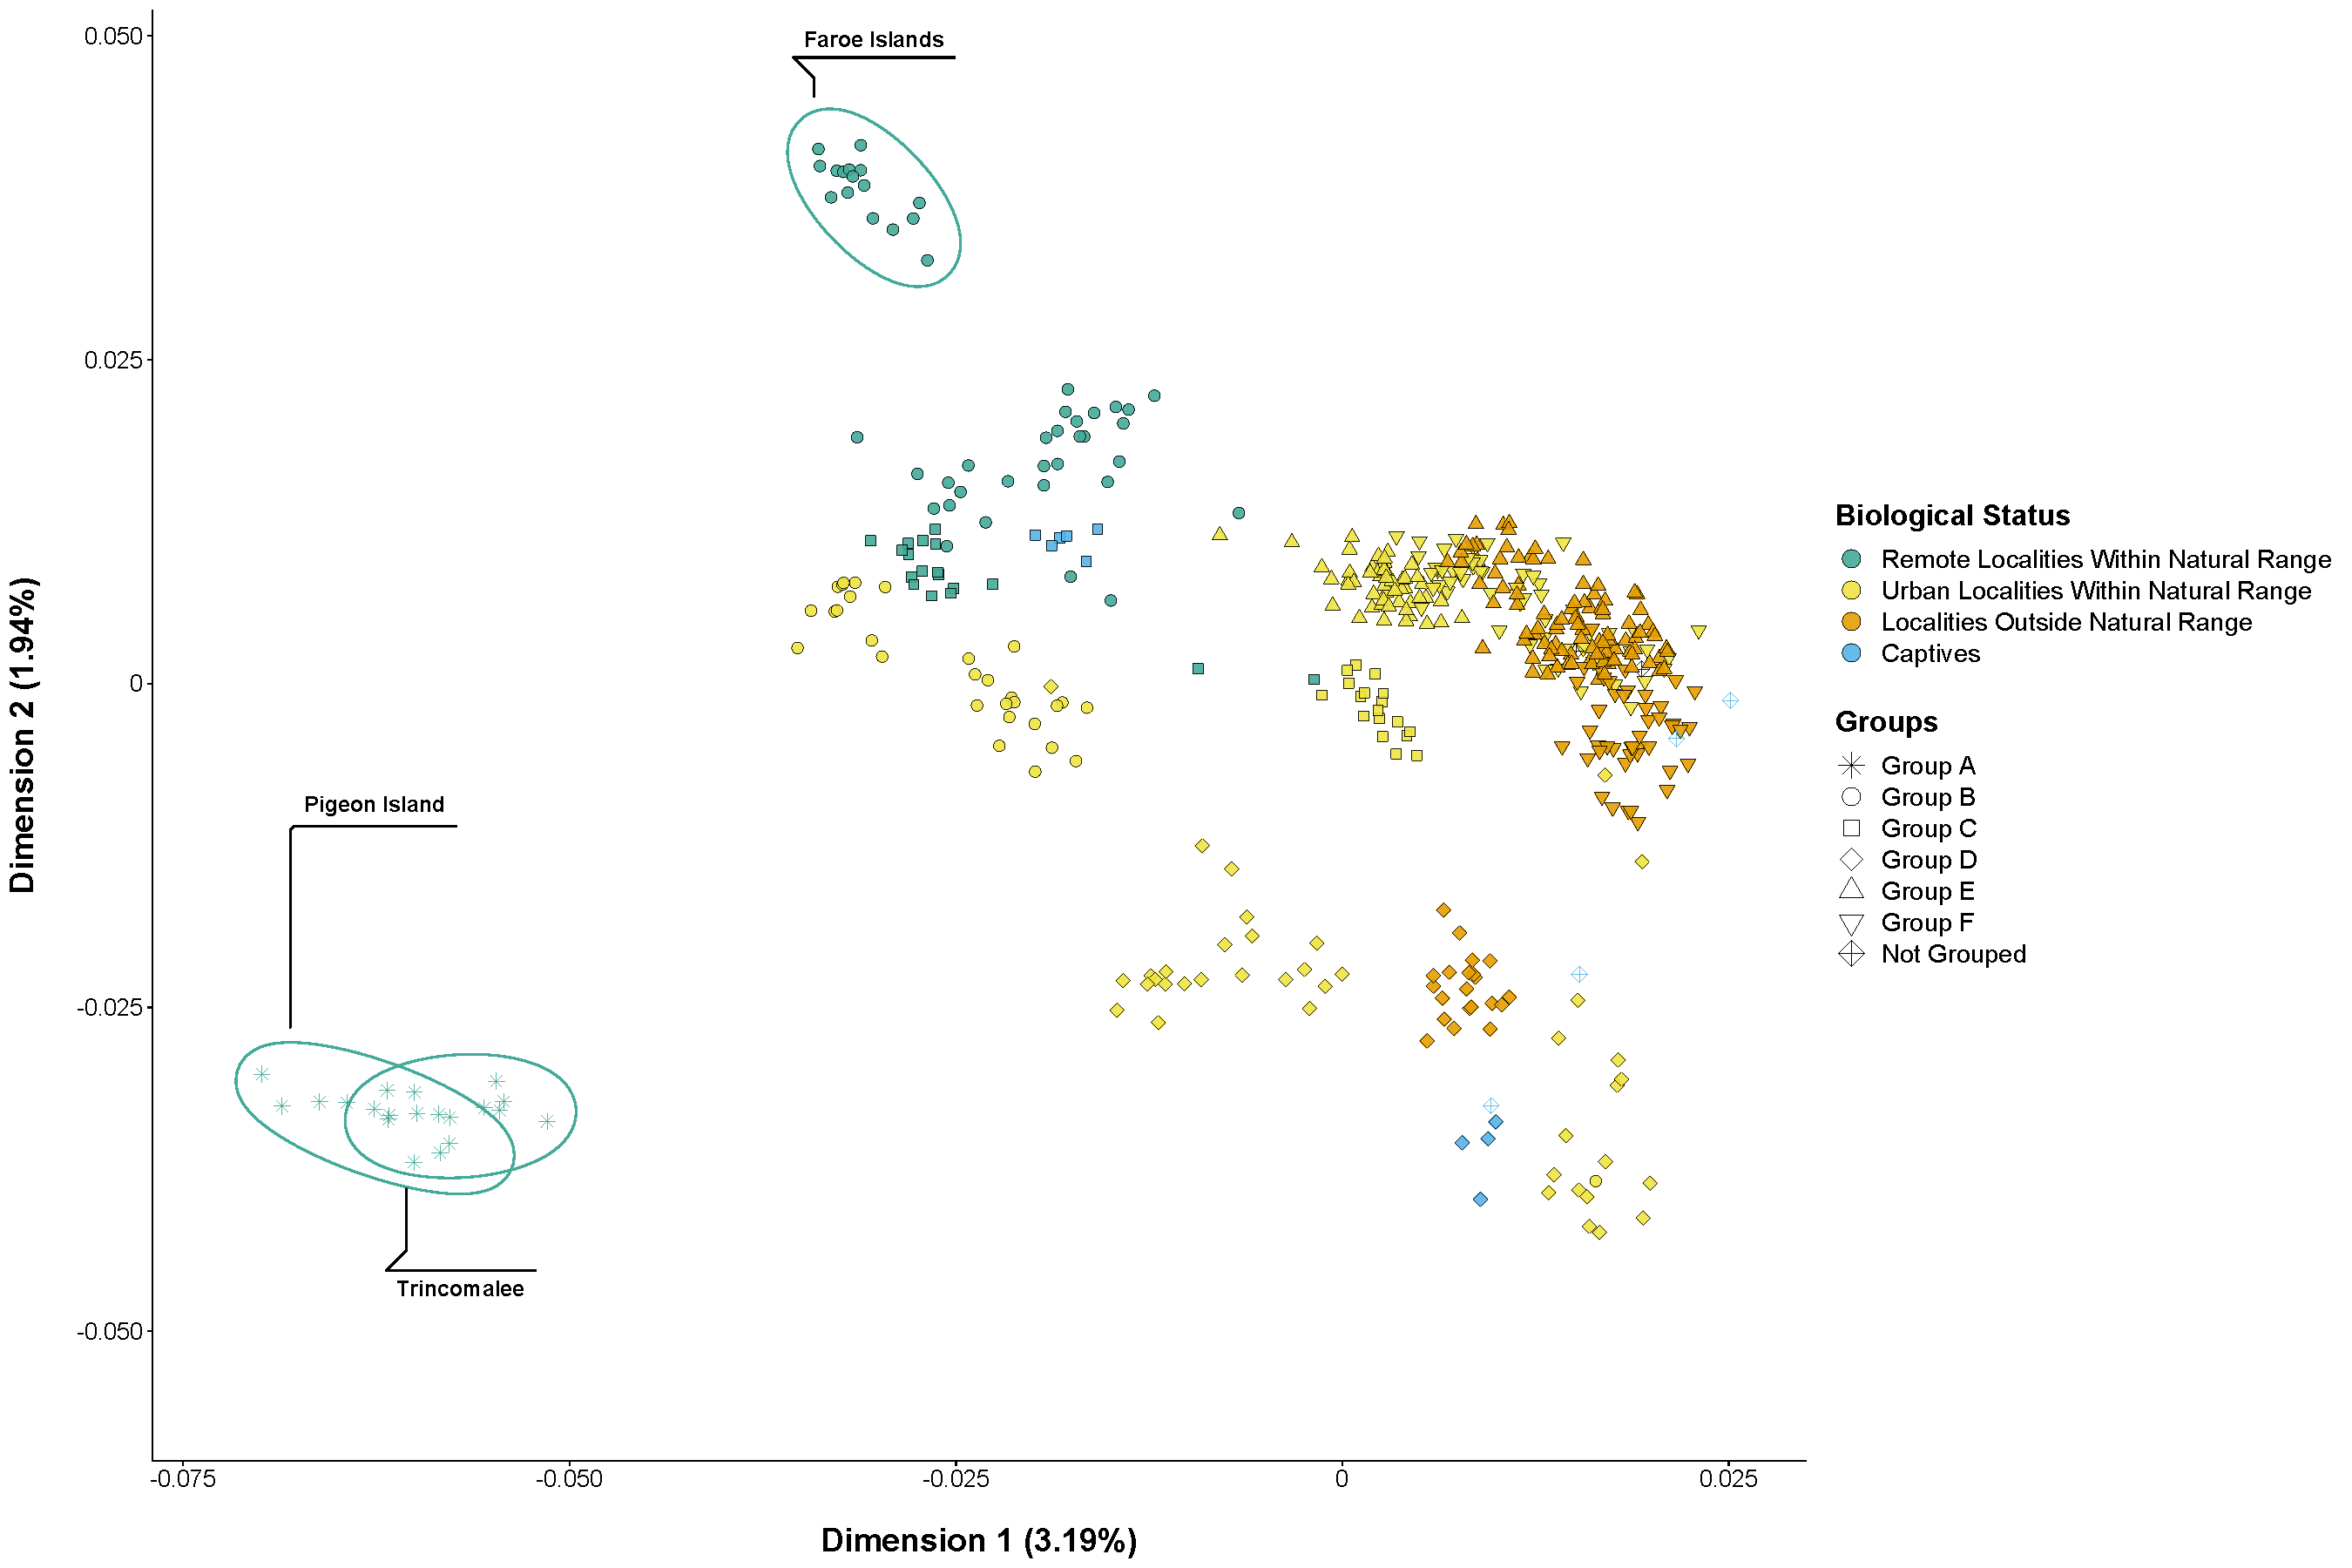
\includegraphics[width=1\textwidth]{../FPG--Plots/FPG--MDS/FPG--MDS_12.pdf}
\caption*{ \scriptsize \textbf{Fig. 2 Map of sampling effort.} This is a trial attempt.}
\label{MainText:FPG--MDS}
\end{figure}

\begin{figure}[!ht]
\centering
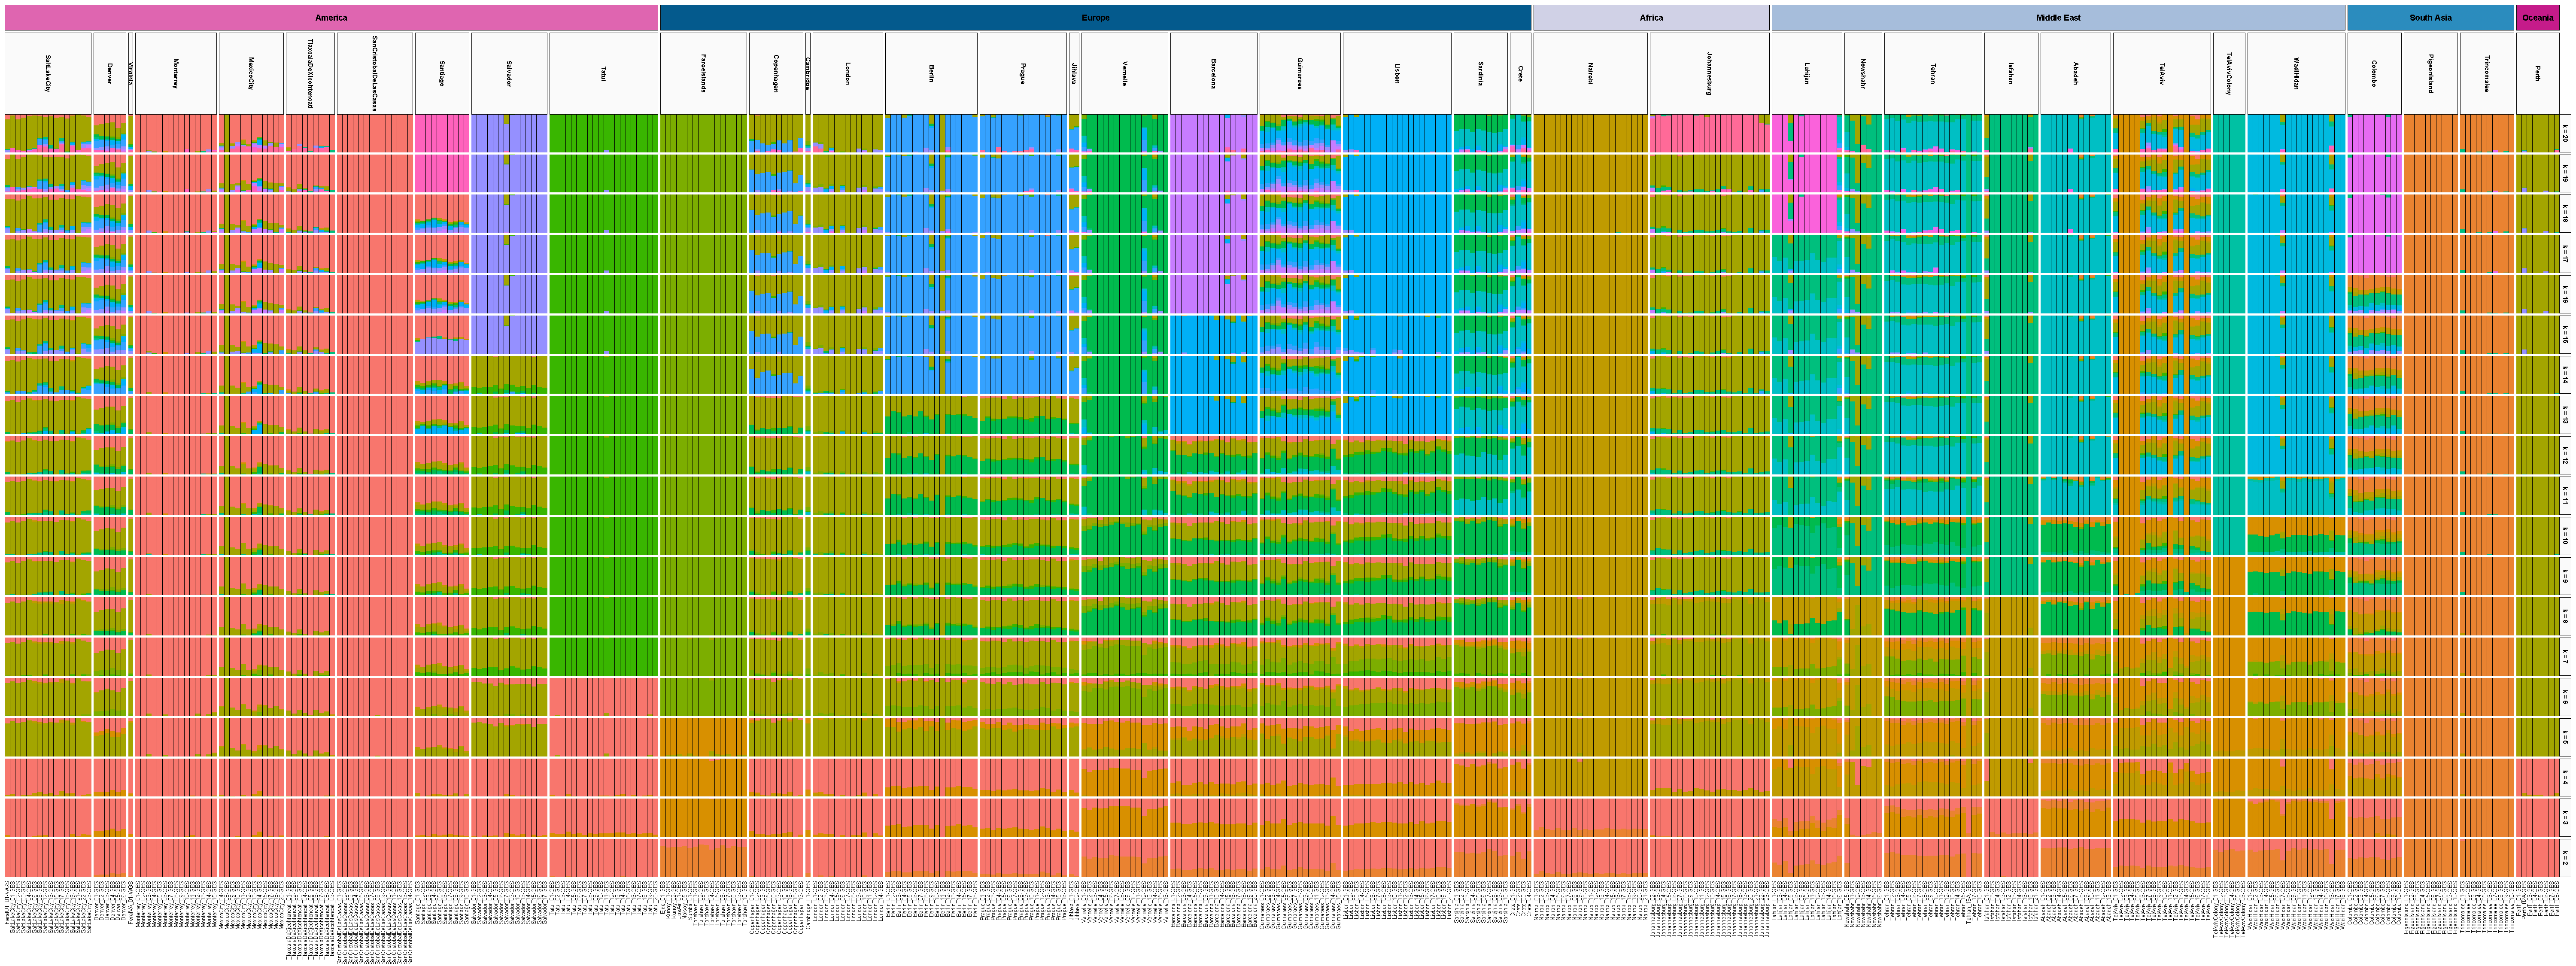
\includegraphics[width=1\textwidth]{../FPG--Plots/FPG--ngsAdmix/FPG--ngsAdmix.pdf}
\caption*{ \scriptsize \textbf{Fig. 3 Map of sampling effort.} This is a trial attempt.}
\label{MainText:FPG--ngsAdmix}
\end{figure}

\newpage
\clearpage

\begin{multicols}{2}
\myheaders{References}
\printbibliography[heading=none]

\hfill

\myheaders{Data Availability} \\
\mytext{All demultiplexed GBS sequencing data is publicly available at SRA (Project Number: PRJNA495951), as well as additional data uploaded to the University of Copenhagen’s long term storage (\url{https://sid.erda.dk/wsgi-bin/ls.py?share_id=aKqQoJvH4Y}).} \\

\myheaders{Acknowledgements} \\
\mytext{We would like to thank our local lab managers Charlotte Hansen, Pernille V. S. Olsen and Tina B. Brand at the Centre for GeoGenetics for their prompt support during the execution of the project. We are grateful to the Cornell University Biotechnology Resource Center for its genotyping services, especially to Sharon E. Mitchell and all lab technicians that worked on this project. Moreover, we deeply thank Gary Jakeman and Kristian Murphy Gregersen for their fieldwork assistance regarding the sampling in England and Denmark, respectively. We also thank Vladimir Orduña for his willingness to let us sample some of the Mexico City pigeons kept at his lab facilities.} \\

\myheaders{Author Contributions} \\
\mytext{M.T.P.G. conceived the project and obtained financial support. M.T.P.G., G.P. and F.G.V. designed the study. G.P. led the project. M.T.P.G., G.P., M.T.O., T.dF.R., P.H., P.N., C.S., I.L-R., S.S.S., K.M., C. L.-F., G.S., R.F., J.D., J. F., N.H., F.K., R. D., A.H., M.B.A. M. C. A.-A. and P. R. E. contributed to sampling. M.D.S. collected and provided the breed samples. G.P. performed the vast majority of DNA extraction and QC. K.M. performed DNA extraction and QC on Sri Lanka samples. G.P. and F.G.V. conducted the computational analyses assisted by M.D.M. G.P., F.G.V., M.T.O and M.T.P.G. interpreted the results. G.P. wrote the first draft of the manuscript with great input from M.T.P.G. and F.G.V. All authors critically reviewed and approved the final manuscript.} \\

\myheaders{Funding} \\
\mytext{This project was funded by Lundbeck Foundation (award R52-5062) and European Research Council (Consolidator grant 681396) granted to MTPG. G.P. was supported by a Danish Government Scholarship and Tuition Fee Waiver Grant provided by the Danish Ministry of Science, Innovation and Higher Education and subsequently by a Ciência Sem Fronteiras Full PhD Abroad Scholarship (Grant Number: 201761/2014-9) provided by the Conselho Nacional de Desenvolvimento Científico e Tecnológico (CNPq) in Brazil.} \\

\myheaders{Competing Interests} \\
\mytext{We have no competing interests.}
\end{multicols}

\end{document}

% 
%%
%%% The END ~~~~